
\chapter{Étude architecturale du projet}
\label{chap:architecture}

\section{Introduction}
\label{sec:introduction}

Ce chapitre présente l'architecture globale du système de collecte de données en temps réel et de gestion des alertes pour les machines en salle de réveil. L'objectif est de décrire les choix technologiques, les composants clés et les interactions entre les différents modules pour répondre aux besoins fonctionnels et non fonctionnels identifiés.

Ce système est conçu pour répondre à un contexte hospitalier sensible, exigeant une haute disponibilité, une sécurité accrue des données, et une capacité d’adaptation à différents environnements techniques.

\section{Architecture globale}
\label{sec:architecture_globale}

Le système VitalSync repose sur une architecture modulaire et évolutive, conçue pour collecter, traiter, stocker et visualiser les données vitales des patients en temps réel. Cette architecture est organisée en trois couches principales, chacune jouant un rôle spécifique dans le traitement des données médicales, comme illustré dans la Figure~\ref{fig:architecture_globale}.

\begin{itemize}
\item \textbf{Couche de collecte des données} : Cette couche est responsable de l'acquisition des données brutes à partir des équipements médicaux. Elle intègre des moniteurs médicaux équipés de caméras IP qui capturent les images des écrans affichant les signes vitaux, tels que la fréquence cardiaque ou la saturation en oxygène (SpO2).

\item \textbf{Couche de traitement et stockage} : Cette couche centralise le traitement des données collectées et leur stockage. Les images capturées sont prétraitées avec OpenCV pour améliorer leur qualité, suivies d'une détection des zones d'intérêt (par exemple, les valeurs des signes vitaux) à l'aide de l'algorithme YOLO. Tesseract OCR extrait ensuite les valeurs numériques ou textuelles des images. Un service Flask gère le traitement des images et communique avec un backend Laravel, qui orchestre la gestion des utilisateurs, des données des patients et des alertes. Une base de données MySQL stocke les informations des patients, les mesures vitales et l'historique des alertes pour un accès rapide et sécurisé.

\item \textbf{Couche de visualisation et notification} : Cette couche permet aux utilisateurs d'interagir avec le système via des interfaces utilisateur modernes. Une application web développée avec React et une application mobile développée avec Flutter offrent un accès aux données des patients et à la gestion des alertes via une API REST. Les notifications en temps réel sont envoyées via Firebase Cloud Messaging (FCM) pour les alertes push sur les appareils mobiles, tandis que les alertes critiques sont transmises par e-mail pour garantir une communication rapide avec le personnel médical.
\end{itemize}

\begin{figure}[H]
\centering
\usetikzlibrary{positioning, fit, shapes.geometric, arrows.meta}
\rotatebox{360}{
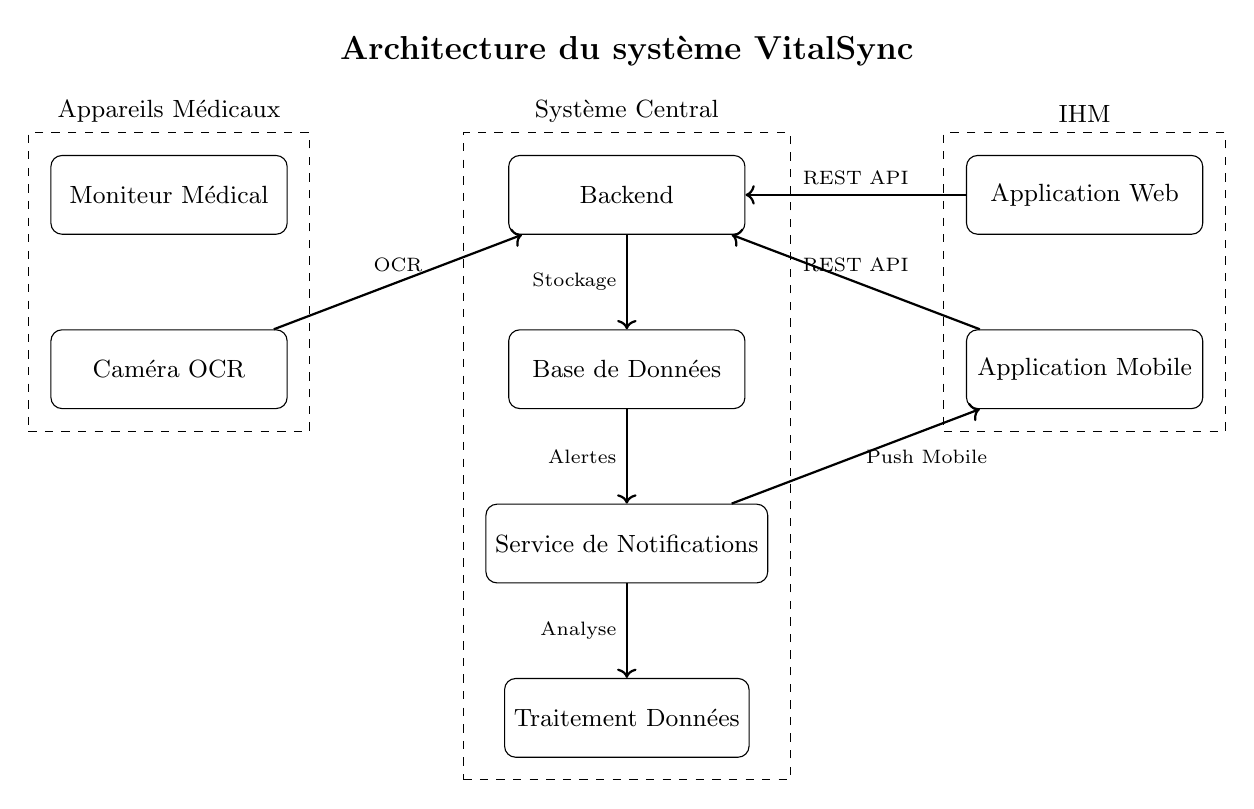
\begin{tikzpicture}[
font=\small,
box/.style={rectangle, draw, rounded corners, minimum width=3cm, minimum height=1cm, align=center},
note/.style={rectangle, draw, text width=3cm, align=left, font=\scriptsize},
arrow/.style={->, thick},
package/.style={rectangle, draw, dashed, inner sep=8pt},
node distance=1.2cm and 2.8cm
]

% --- Bloc central : Backend et services ---
\node[box] (backend) {Backend};
\node[box, below=of backend] (database) {Base de Données};
\node[box, below=of database] (notifications) {Service de Notifications};
\node[box, below=of notifications] (processing) {Traitement Données};
\node[package, fit=(backend) (database) (notifications) (processing), label=above:Système Central] {};

% --- Bloc gauche : Appareils Médicaux ---
\node[box, left=of backend] (monitor) {Moniteur Médical};
\node[box, below=of monitor] (camera) {Caméra OCR};
\node[package, fit=(monitor) (camera), label=above:Appareils Médicaux] {};

% --- Bloc droit : Interfaces ---
\node[box, right=of backend] (webapp) {Application Web};
\node[box, below=of webapp] (mobileapp) {Application Mobile};
\node[package, fit=(webapp) (mobileapp), label=above:IHM] {};

% --- Flèches de liaison ---
\draw[arrow] (camera) -- (backend) node[midway, above, font=\scriptsize] {OCR};
\draw[arrow] (webapp) -- (backend) node[midway, above, font=\scriptsize] {REST API};
\draw[arrow] (mobileapp) -- (backend) node[midway, above, font=\scriptsize] {REST API};
\draw[arrow] (backend) -- (database) node[midway, left, font=\scriptsize] {Stockage};
\draw[arrow] (database) -- (notifications) node[midway, left, font=\scriptsize] {Alertes};
\draw[arrow] (notifications) -- (processing) node[midway, left, font=\scriptsize] {Analyse};
\draw[arrow] (notifications) -- (mobileapp) node[midway, right, font=\scriptsize] {Push Mobile};

% --- Titre ---
\node[above=1cm of backend, font=\bfseries\large] {Architecture du système VitalSync};

\end{tikzpicture}
}
\caption{Architecture globale}
\label{fig:architecture_globale}
\end{figure}

La Figure~\ref{fig:architecture_globale} présente une vue d'ensemble de l'architecture du système VitalSync, mettant en évidence les interactions entre les différentes couches. Le bloc "Appareils Médicaux" regroupe les moniteurs médicaux et les caméras OCR, qui capturent les données brutes sous forme d'images. Ces images sont transmises au bloc "Système Central" via un flux OCR, où elles sont traitées par des algorithmes (OpenCV, YOLO, Tesseract) pour extraire les signes vitaux. Le backend Laravel coordonne les opérations, stocke les données dans une base MySQL et gère les alertes via un service de notifications. Les interfaces utilisateur (web et mobile) accèdent aux données via des API REST, tandis que les notifications push (FCM) et les e-mails assurent une communication rapide des alertes critiques. Cette architecture garantit une intégration fluide des composants, une scalabilité pour gérer un grand volume de données et une réactivité pour les alertes en temps réel.

\subsection{Diagramme de classes}
\label{subsec:classes}
Le système VitalSync utilise une base de données MySQL pour stocker les données des patients, les signes vitaux et les alertes. Le diagramme de classes (Figure~\ref{fig:class_diagram}) illustre le schéma de la base de données, incluant les entités clés (par exemple, Patient, Mesure, Alerte) et leurs relations. Ce schéma garantit une structure relationnelle robuste pour la gestion des données. Pour les détails d'implémentation, voir le Chapitre~\ref{chap:sprint1}.

\begin{figure}[H]
\centering
\rotatebox{90}{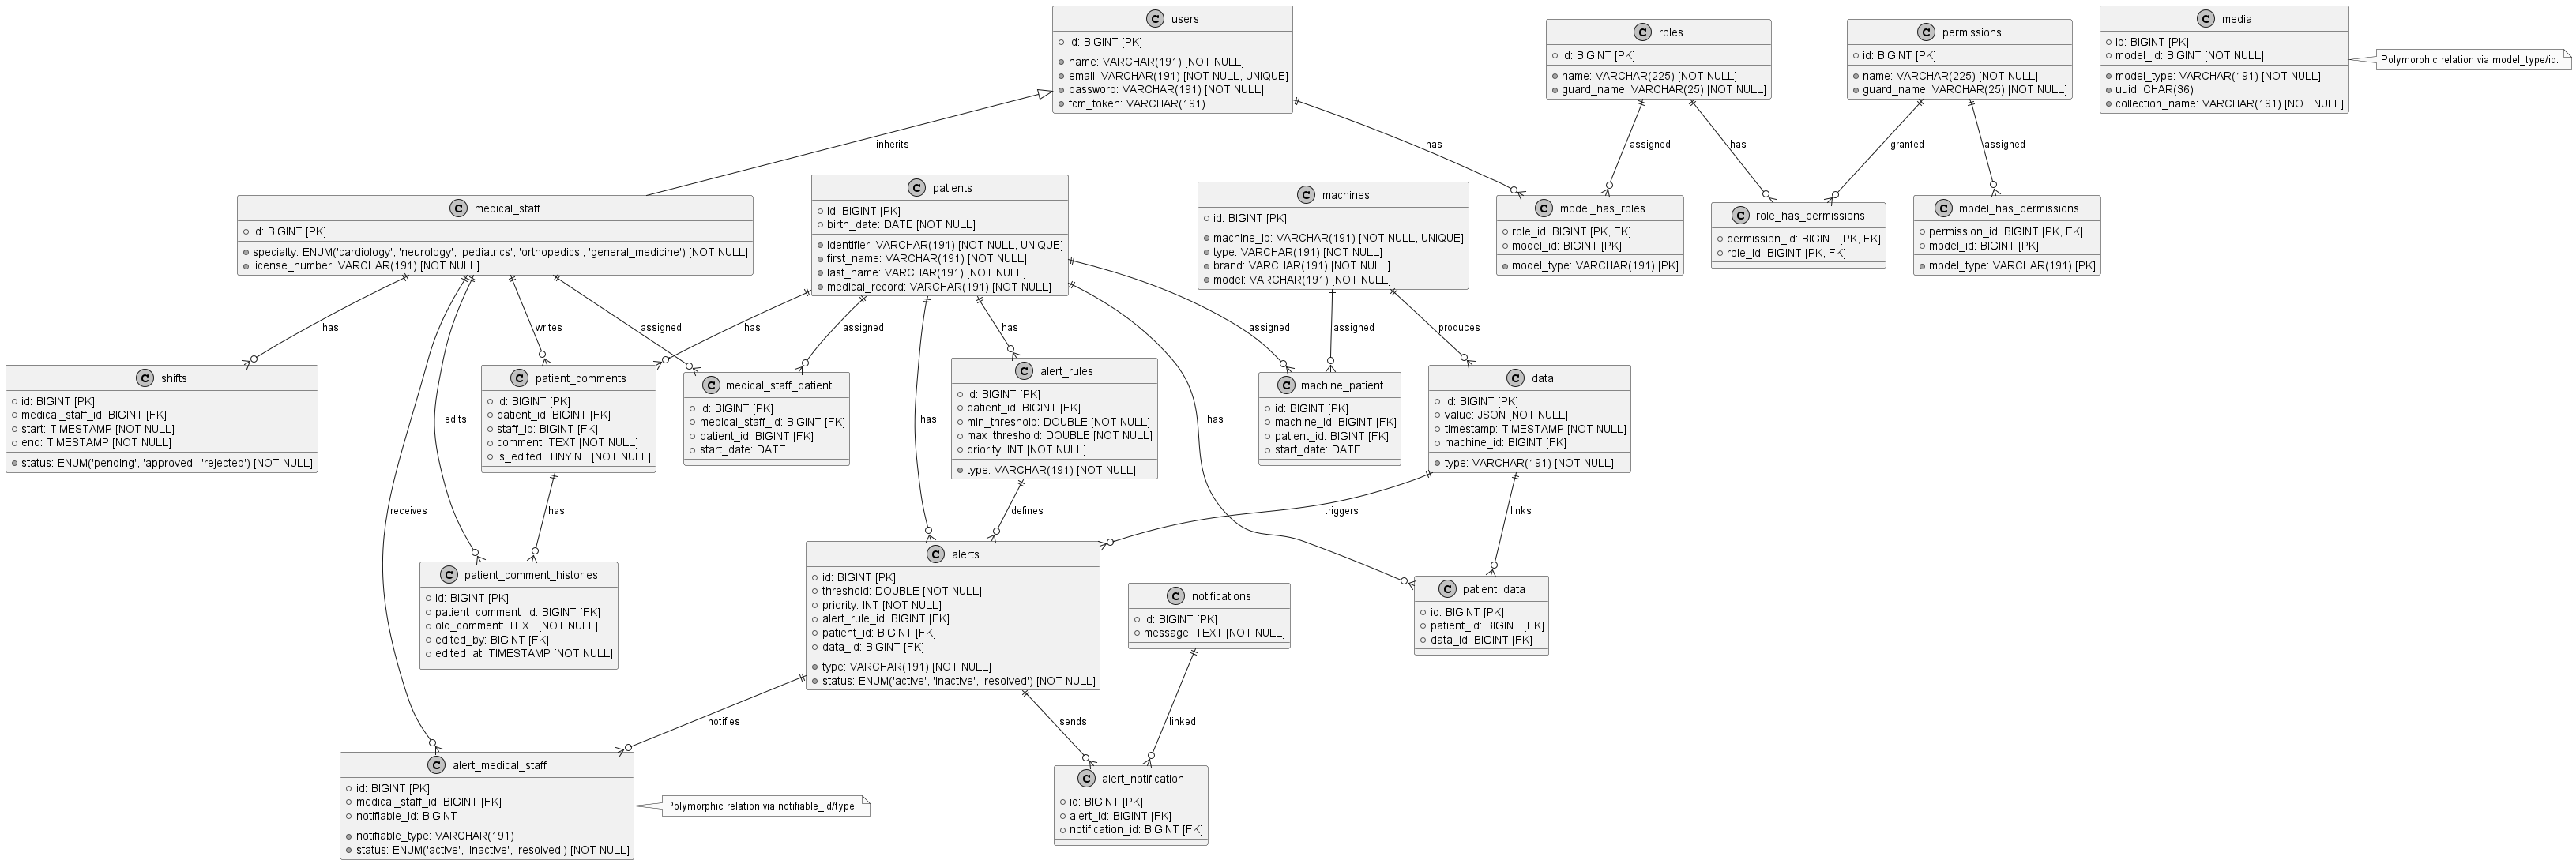
\includegraphics[width=1.5\textwidth]{chapter3/diagrams/class.png}}
\caption{Diagramme de classes}
\label{fig:class_diagram}
\end{figure}

\subsection{Diagramme de séquence}
Le système VitalSync traite les signes vitaux en temps réel, depuis la capture des images par les caméras jusqu'à la notification du personnel médical via FCM. Le diagramme de séquence (Figure~\ref{fig:global_sequence_diagram}) illustre le workflow global, mettant en évidence les interactions entre la caméra, le traitement YOLOv8, le système d'alerte et le système de notification. Ce workflow garantit une chaîne de traitement efficace et réactive. Pour les détails d'implémentation du Sprint 1, voir le Chapitre~\ref{chap:sprint1}.

\begin{figure}[H]
\centering
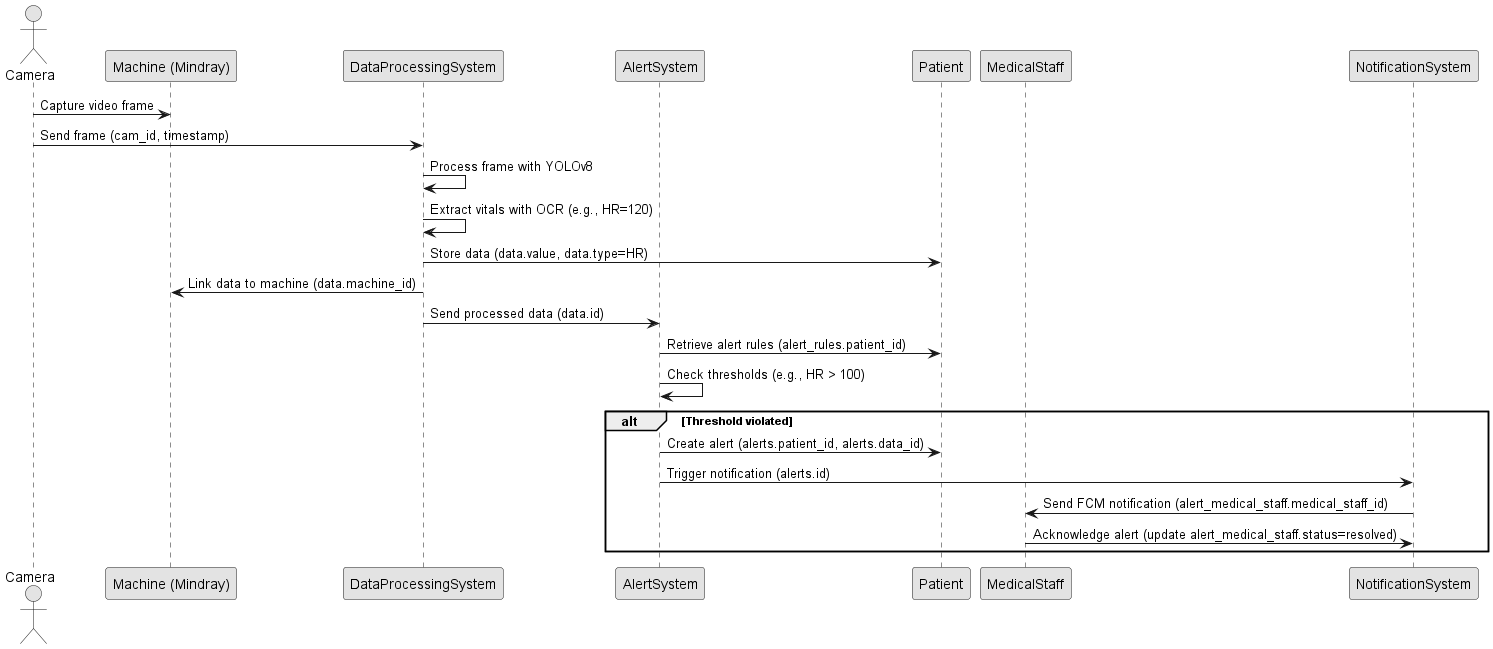
\includegraphics[width=0.9\textwidth]{chapter3/diagrams/sequence.png}
\caption{Diagramme de séquence global}
\label{fig:global_sequence_diagram}
\end{figure}
% \section{Diagrammes d'architecture}
% \label{sec:diagrammes}

\subsection{Diagramme de déploiement}
\label{subsec:deploiement}

Le système VitalSync s'appuie sur une architecture distribuée qui intègre des dispositifs médicaux, des serveurs applicatifs, des services de traitement d'images et des interfaces utilisateur. Cette architecture est structurée en couches distinctes, chacune hébergeant des composants matériels et logiciels spécifiques, comme illustré dans la Figure~\ref{fig:diagramme_deploiement}. Les sections suivantes décrivent les rôles et les interactions des composants au sein de chaque couche, ainsi que l'infrastructure réseau et les protocoles de communication qui assurent leur interconnexion.

\paragraph{Couche de collecte des données}
La couche de collecte des données est dédiée à l'acquisition des informations vitales des patients. Elle comprend des moniteurs médicaux qui mesurent en continu les signes vitaux, tels que la fréquence cardiaque ou la saturation en oxygène (SpO2). Ces moniteurs sont associés à des caméras IP qui capturent les écrans affichant ces données sous forme d'images. Les images capturées sont ensuite transmises au système central pour traitement, garantissant une collecte précise et en temps réel des données brutes.

\paragraph{Couche de traitement et stockage}
La couche de traitement et stockage constitue le cœur fonctionnel du système, hébergé sur un serveur central. Ce serveur exécute l'API Laravel pour la gestion des utilisateurs, des données des patients et des alertes, ainsi qu'un service Flask dédié au traitement des images. Le traitement des images s'appuie sur plusieurs technologies : OpenCV effectue un prétraitement pour améliorer la qualité des images, YOLO détecte les régions d'intérêt (par exemple, les zones affichant les valeurs vitales), et Tesseract OCR extrait les données textuelles ou numériques de ces régions. Une base de données MySQL stocke les informations des patients, les mesures vitales et l'historique des alertes, offrant un accès rapide et sécurisé aux données pour les analyses et les rapports.

\paragraph{Couche de visualisation et notification}
La couche de visualisation et notification permet au personnel médical d'interagir avec le système et de recevoir des alertes en temps réel. Une application mobile développée avec Flutter offre une interface pour consulter les données des patients et gérer les alertes directement sur les appareils mobiles. De même, une application web basée sur React fournit une interface utilisateur complète pour le personnel médical, accessible via des navigateurs. Les notifications en temps réel sont gérées par Firebase Cloud Messaging (FCM), qui envoie des alertes push aux appareils mobiles pour signaler des événements critiques, garantissant une réactivité immédiate.

\paragraph{Infrastructure et support}
L'infrastructure réseau joue un rôle essentiel dans la connectivité et la sécurité du système. Un réseau sécurisé, basé sur des protocoles HTTPS et des mécanismes d'authentification comme Sanctum, assure une communication fiable et protégée entre tous les composants, qu'ils soient locaux ou déployés dans le cloud. Cette infrastructure garantit l'intégrité des données et la confidentialité des informations médicales tout au long du flux de traitement.

\paragraph{Connexions et protocoles}
Les interactions entre les composants s'appuient sur des protocoles standardisés pour assurer une communication fluide et sécurisée. Les interfaces web et mobile communiquent avec le serveur backend via une API REST basée sur HTTP/HTTPS, complétée par des WebSockets pour les mises à jour en temps réel. Les flux vidéo provenant des caméras IP sont traités localement ou dans le cloud, où YOLO et Tesseract OCR analysent les images pour extraire les données vitales. Les alertes critiques sont diffusées via Firebase Cloud Messaging (FCM), permettant une notification rapide et fiable du personnel médical.

\begin{figure}[H]
    \centering
    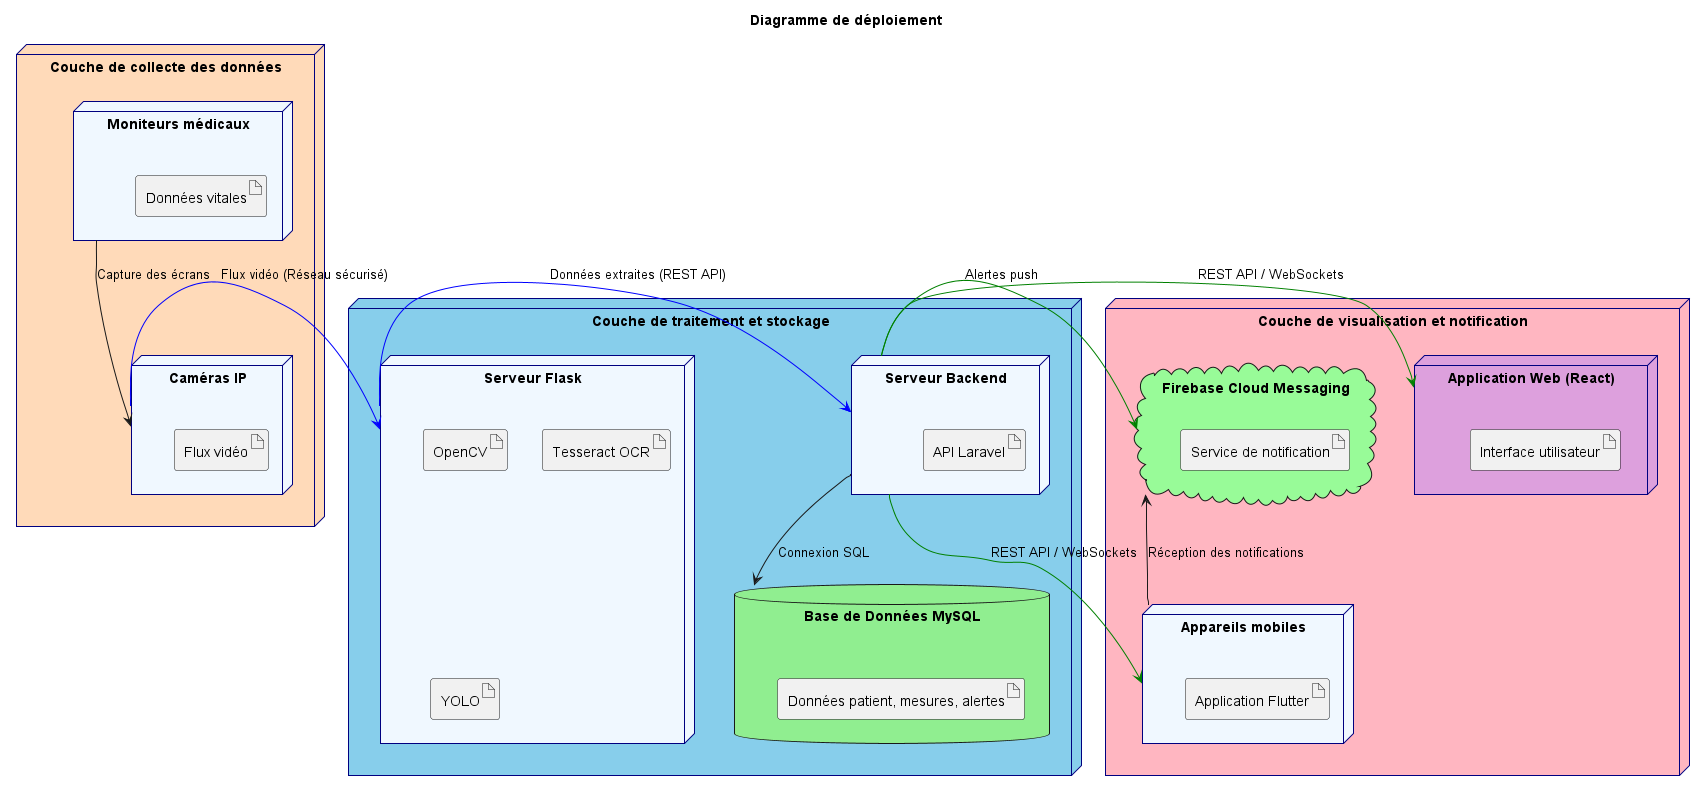
\includegraphics[width=0.8\textwidth]{chapter3/diagrams/deployment_diagram.png}
    \caption{Diagramme de déploiement}
    \label{fig:diagramme_deploiement}
\end{figure}

    La Figure~\ref{fig:diagramme_deploiement} illustre le déploiement des composants du système VitalSync à travers son architecture distribuée. Les moniteurs médicaux et les caméras IP, regroupés dans la couche de collecte, transmettent les images des signes vitaux au serveur central. Ce dernier, au sein de la couche de traitement et stockage, exécute les services Flask pour le traitement d'images (YOLO, OpenCV, Tesseract) et l'API Laravel pour la gestion des données, stockées dans une base MySQL. Les interfaces utilisateur, déployées sur des appareils mobiles (Flutter) et des navigateurs (React), accèdent aux données via une API REST et reçoivent des notifications push via FCM. Un réseau sécurisé relie tous les composants, assurant une communication rapide, fiable et protégée. Cette organisation permet une scalabilité et une robustesse adaptées aux besoins des environnements médicaux critiques.
    
    
\subsection{Diagramme de composants}
\label{subsec:composants}

The backend of the system is designed to handle core functionalities through a combination of robust technologies. Python modules are utilized for advanced data processing, including the detection of data zones using the YOLO algorithm, optical character recognition (OCR) with Tesseract, and comprehensive data analysis. Additionally, Laravel services manage critical operations such as user authentication, alert management, and notification delivery, ensuring secure and efficient backend performance.

The frontend provides an intuitive and responsive user experience through two primary interfaces. React-based dashboards enable effective visualization of data, offering users clear and interactive insights into the processed information. Complementing this, a Flutter application delivers mobile alerts, allowing users to receive timely notifications and stay informed on the go.

\begin{figure}[H]
\centering
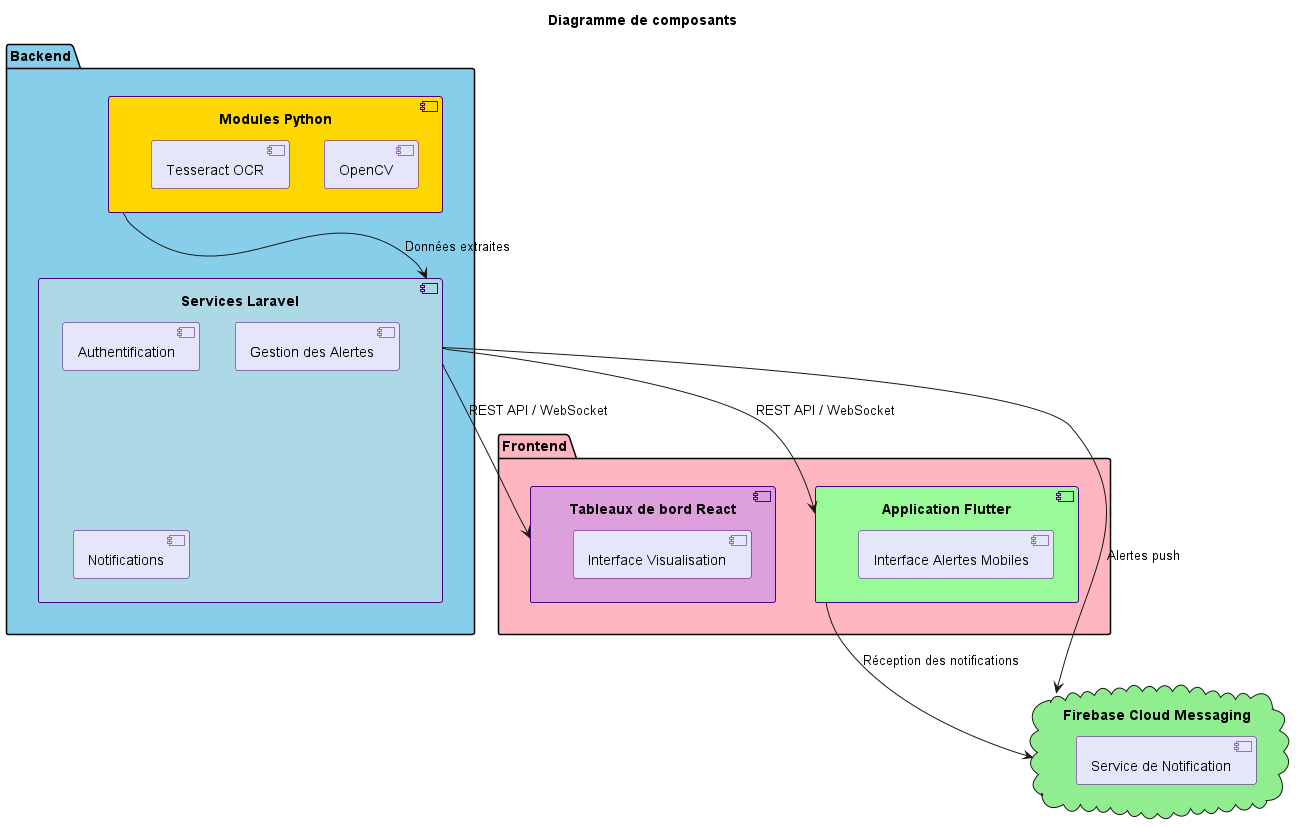
\includegraphics[width=0.8\textwidth]{chapter3/diagrams/component_diagram.png}
\caption{Diagramme de composants du système}
\label{fig:composants}
\end{figure}

\subsection{Diagramme d'activité}
\label{subsec:diagramme_activite}


Le diagramme d'activité présenté dans la Figure~\ref{fig:activity_flux_donnees} illustre les différentes étapes du traitement des données au sein du système VitalSync, depuis la collecte des données jusqu’à la notification des alertes. Il met en évidence les actions séquentielles réalisées par les différents modules, en soulignant les conditions qui déclenchent des alertes médicales. Cette représentation permet de visualiser clairement le parcours des données capturées par les caméras IP, traitées par les services intelligents (YOLO, OpenCV, Tesseract), puis analysées par le backend afin de détecter d’éventuelles anomalies. En cas de dépassement de seuils critiques, une alerte est générée et transmise en temps réel au personnel médical via des interfaces web et mobiles, garantissant ainsi une intervention rapide et efficace.

\begin{figure}[H]
    \centering
    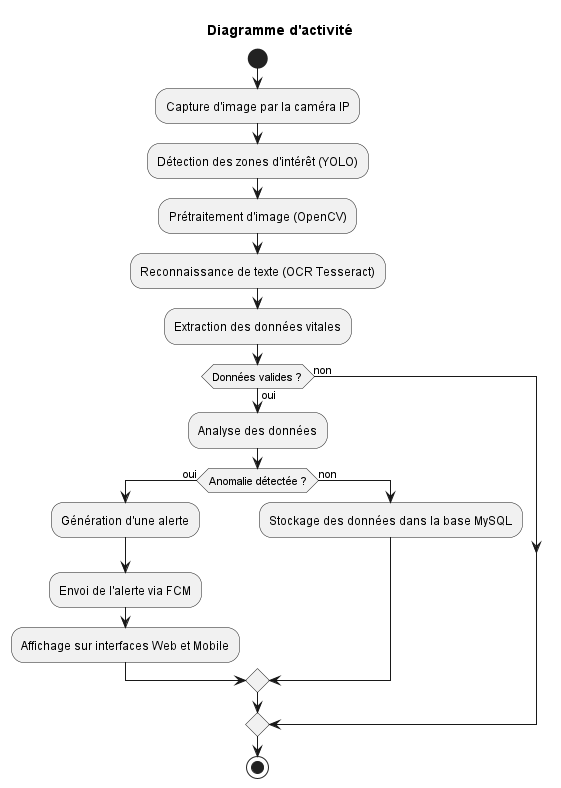
\includegraphics[width=0.75\textwidth]{chapter3/diagrams/activity_dataflow.png}
    \caption{Diagramme d'activité du flux de données}
    \label{fig:activity_flux_donnees}
\end{figure}

\section{Architecture physique et fonctionnement}  
\label{sec:architecture_physique}  

\subsection{Composants matériels}  
\label{subsec:composants_materiels}  

Les composants matériels du système sont conçus pour faciliter une collecte, un traitement et une communication efficaces des données. Les moniteurs médicaux recueillent des données vitales telles que la fréquence cardiaque, la tension artérielle et la saturation en oxygène, affichant ces mesures sur leurs écrans. Les caméras capturent ces écrans et transmettent les images au service de traitement, où les technologies YOLO et OCR analysent les données.  

Les serveurs, hébergés localement, stockent et traitent ces données en exécutant YOLO, OpenCV et Tesseract pour l'analyse d'images. Un réseau de communication sécurisé assure la transmission fiable des données entre les moniteurs, les caméras, les serveurs et les applications. Les appareils mobiles permettent au personnel médical de recevoir des notifications push en temps réel et d'accéder aux données vitales, améliorant ainsi la réactivité.  

\subsection{Fonctionnement}  
\label{subsec:fonctionnement}  

Le système fonctionne en trois étapes principales : collecte des données, traitement des données et génération d'alertes. Durant l'étape de collecte, les caméras capturent les écrans des moniteurs médicaux, et le modèle YOLO identifie les zones de données, telles que la fréquence cardiaque ou la SpO2. Ces images sont prétraitées avec OpenCV, et Tesseract OCR extrait les valeurs des signes vitaux.

Lors de l'étape de traitement, le système analyse les données en temps réel pour détecter les anomalies en les comparant à des seuils prédéfinis, stockant les résultats dans une base de données MySQL pour une analyse ultérieure. Enfin, lors de la génération d'alertes, celles-ci sont déclenchées lorsque les seuils sont dépassés et sont envoyées au personnel médical via FCM, tout en étant affichées sur les interfaces web et mobiles pour un accès immédiat.  

\subsection{Spécifications logicielles}  
\label{subsec:spec_logiciels}  

L'architecture logicielle est composée de plusieurs éléments intégrés pour garantir une fonctionnalité robuste. Le backend utilise Laravel pour gérer l'authentification des utilisateurs, la manipulation des données et les services de notification via FCM, tandis que Python gère le traitement des données, intégrant YOLO pour la détection des zones de données, l'OCR avec OpenCV et Tesseract, ainsi que l'analyse d'images.  

L'interface frontend comprend une interface web basée sur React pour la visualisation interactive des données et la gestion des alertes, complétée par une application mobile Flutter pour les notifications en temps réel et l'accès aux données. Une base de données MySQL stocke les données des patients, les alertes et les historiques. La communication est facilitée par des API REST pour les interactions entre le frontend, le backend et l'application mobile, avec WebSockets permettant des notifications en temps réel.  

Parmi les outils supplémentaires figurent YOLOv8 intégré avec PyTorch pour la détection des zones de données, Docker pour la conteneurisation, Git pour le contrôle de version et Swagger pour le test des API REST.  

\subsection{Flux de communication}  
\label{subsec:flux_communication}  

Le flux de communication commence par la collecte des données depuis les moniteurs médicaux, où YOLO détecte les zones de données et l'OCR extrait les informations pertinentes. Les données sont transmises de manière sécurisée au backend via un réseau protégé. Le backend traite les données en temps réel, les stocke dans une base de données MySQL et génère des alertes si des anomalies sont détectées.  

Ces alertes sont envoyées au personnel médical via FCM. Les utilisateurs peuvent accéder aux données et aux alertes via l'application web ou mobile, assurant une communication fluide et rapide à travers le système.  

\begin{figure}[H]  
    \centering  
    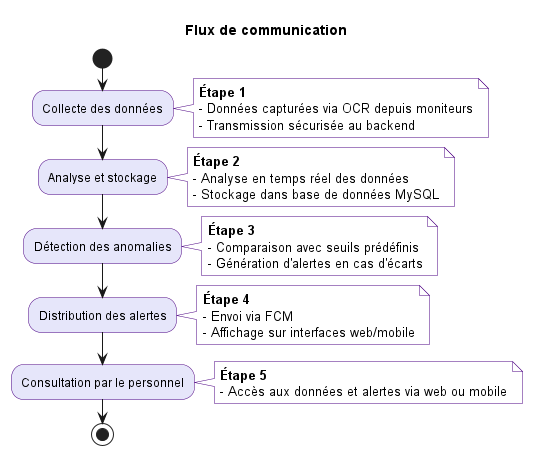
\includegraphics[width=0.9\textwidth]{chapter3/diagrams/communication_flow_chart.png}  
    \caption{Schéma général du flux de communication}  
    \label{fig:flux_communication}  
\end{figure}  

\section{Justification de l'architecture}  
\label{sec:justification_architecture}  

L'architecture proposée garantit plusieurs qualités essentielles. Sa conception modulaire sépare le système en couches distinctes — collecte avec YOLO, traitement et notification — facilitant la maintenance et l'évolutivité. Le système assure une grande réactivité en fournissant des alertes en temps réel, soutenu par une détection précise des zones de données via YOLO, permettant des réponses rapides aux situations critiques.  

L'interopérabilité est maintenue grâce à la compatibilité avec YOLO, l'OCR et les standards d'échange de données médicales, assurant une intégration transparente avec les systèmes existants. De plus, l'architecture offre une flexibilité, permettant un déploiement sur des serveurs locaux ou cloud pour répondre aux besoins variés des hôpitaux.  

\section{Conclusion}  
\label{sec:conclusion}  

L'architecture proposée, renforcée par l'intégration de YOLO pour une détection précise des zones de données, garantit une collecte fiable des données, un traitement efficace et une diffusion rapide des alertes tout en respectant les contraintes de sécurité et d'interopérabilité. Sa conception modulaire permet des améliorations futures, telles que l'intégration de nouveaux dispositifs ou l'ajout de fonctionnalités analytiques avancées, en faisant une solution robuste et adaptable pour la surveillance médicale.